\documentclass[10pt,a4paper,UTF8,fontset=fandol]{ctexart}

\usepackage[top=20mm,bottom=20mm,left=20mm,right=20mm,headheight=20pt,headsep=5mm,footskip=8mm]{geometry}
\usepackage{graphicx}
\usepackage{capt-of}
\usepackage{booktabs}
\usepackage{tabularx}
\usepackage{xcolor}
\usepackage{tikz}
\usepackage{enumitem}
\usepackage{fancyhdr}
\usepackage[hidelinks]{hyperref}

\usetikzlibrary{arrows.meta,positioning,shapes.geometric,calc}

% v1.0.1 发行包及默认种子 17 的仿真记录
\newcommand{\ReleaseSize}{38.62\,MiB}
\newcommand{\ReleaseBytes}{40\,491\,008}
\newcommand{\MapCoverage}{93.08\%}
\newcommand{\MapVersion}{V1034}
\newcommand{\MapTime}{344\,秒}

% 深青、灰、白配色体系
\definecolor{DeepTeal}{HTML}{0F5257}
\definecolor{MidTeal}{HTML}{1B7278}
\definecolor{TealTint}{HTML}{ECF4F5}
\definecolor{SlateText}{HTML}{1E293B}
\definecolor{MutedGray}{HTML}{64748B}
\definecolor{RuleGray}{HTML}{CBD5E1}
\definecolor{LightPanel}{HTML}{F8FAFC}
\definecolor{WarnSlate}{HTML}{475569}
\definecolor{WarnTint}{HTML}{F1F5F9}

\color{SlateText}

% 章节与版式设定
\ctexset{
  section = {
    format = \Large\bfseries\color{DeepTeal},
    name = {,},
    number = \arabic{section},
    aftername = \hspace{0.6em},
    beforeskip = 8pt plus 2pt minus 2pt,
    afterskip = 6pt plus 2pt minus 1pt,
  },
  subsection = {
    format = \normalsize\bfseries\color{MidTeal},
    beforeskip = 6pt plus 1pt minus 1pt,
    afterskip = 3pt plus 1pt minus 1pt,
  }
}

\pagestyle{fancy}
\fancyhf{}
\fancyhead[L]{\footnotesize\color{MutedGray}工厂机器人协同作业平台软件开发日志}
\fancyhead[R]{\footnotesize\color{MutedGray}Factory Robot Collaboration Platform}
\fancyfoot[C]{\footnotesize\color{MutedGray}第 \thepage{} 页}
\renewcommand{\headrulewidth}{0.4pt}
\renewcommand{\headrule}{\hbox to\headwidth{\color{RuleGray}\leaders\hrule height \headrulewidth\hfill}}
\renewcommand{\footrulewidth}{0pt}

\fancypagestyle{firstpage}{
  \fancyhf{}
  \fancyfoot[C]{\footnotesize\color{MutedGray}第 \thepage{} 页}
  \renewcommand{\headrulewidth}{0pt}
  \renewcommand{\footrulewidth}{0pt}
}

\setlist[itemize]{leftmargin=1.4em,itemsep=2pt,topsep=3pt,parsep=0pt}
\renewcommand{\arraystretch}{1.22}
\setlength{\parindent}{2em}
\setlength{\parskip}{3pt}

\hypersetup{
  pdftitle={工厂机器人协同作业平台软件开发日志},
  pdfauthor={朱华天，GPT-6.2 Sol，Gemini 4 Neon},
  colorlinks=true,
  linkcolor=DeepTeal,
  citecolor=DeepTeal,
  urlcolor=DeepTeal
}

\begin{document}
\thispagestyle{firstpage}

% 首页抬头（非独立封面，直接接正文）
\noindent

\begin{tikzpicture}
  \fill[DeepTeal] (0,0) rectangle (\textwidth, 1.8pt);
\end{tikzpicture}
\vspace{4pt}

\begin{flushleft}
  {\LARGE\bfseries\color{DeepTeal} 工厂机器人协同作业平台软件开发日志}\\[4pt]
  {\small\color{MutedGray} Factory Robot Collaboration Platform}\\[6pt]
  {\normalsize\color{SlateText} 朱华天，GPT-6.2 Sol，Gemini 4 Neon}\\[2pt]
  {\small\color{MutedGray} 2026年11月25日}\\[2pt]
  {\small \url{https://github.com/ZHT1235456/factory-robot-collaboration-platform}}
\end{flushleft}

\vspace{2pt}
\noindent{\color{RuleGray}\hrule height 0.5pt}
\vspace{6pt}

\noindent\colorbox{TealTint}{%
  \parbox{\dimexpr\textwidth-2\fboxsep\relax}{%
    \small{\bfseries\color{DeepTeal} 简介}\hspace{0.6em}本文记录工厂机器人协同作业平台桌面仿真软件（v1.0.1）的设计与开发过程。软件面向循环水公用工程厂房的联动检修任务，基于桌面应用框架 Tauri、三维渲染引擎 Three.js、物理仿真引擎 MuJoCo 与神经网络推理引擎 ONNX Runtime 搭建，支持四足机器人 Go2 与人形机器人 G1 联合完成下层建图、地图交付、路径规划与设备检修。%
  }%
}
\vspace{4pt}

\section{厂房场景与软件发布}

\subsection{厂房场景与双机协同}

这款桌面软件模拟 Go2 和 G1 在循环水厂房协作检修。厂房长 47.2\,m、宽 26\,m，中央泵房设有夹层和楼梯。Go2 负责下层建图，也能进入低位通道查看仪表和指示片。G1 核对高处的设备编号，并用手开盖、取放备件和操作按钮。

两台机器人通过消息交接地图、确认何时可以进入下一道工序。三维场景用气泡显示这些消息。整套流程共 5 张工单、30 个任务节点，依次是泵组测振、过滤隔离、换热复检、备件转运和回水验收。

\subsection{桌面端发布说明}

v1.0.1 提供 Windows x64 单文件可执行程序，体积为 \ReleaseSize{}（\ReleaseBytes{} 字节）。界面由 Microsoft Edge WebView2 显示。双击启动后默认全屏，按 \texttt{F11} 可切换窗口模式。图~\ref{fig:handoff} 记录了 G1 接图后的界面。

\begin{figure}[htbp]
  \centering
  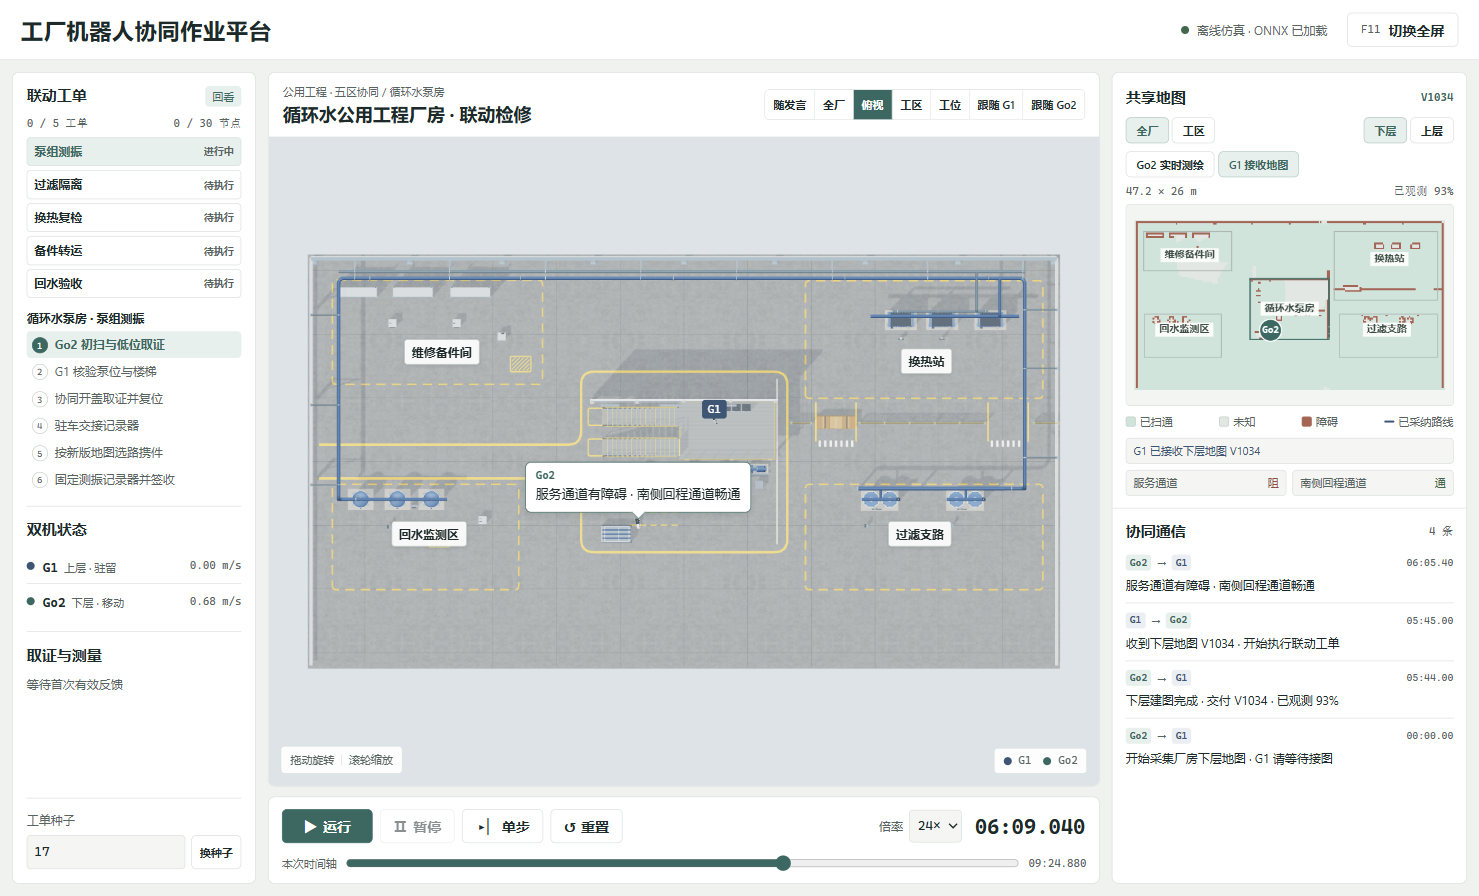
\includegraphics[width=\linewidth,height=0.33\textheight,keepaspectratio]{../assets/factory-map-handoff.png}
  \caption{G1 接图后的界面。左侧列出工单和机器人状态，右侧可切换 Go2 的实时地图和 G1 收到的版本。}
  \label{fig:handoff}
\end{figure}

\clearpage

\section{技术栈与进程通信}

\subsection{桌面架构与进程通信}

图~\ref{fig:arch} 列出了桌面界面、Rust 宿主和 Python 仿真进程之间的关系。首次启动时，Rust 宿主把 PyInstaller 打包的仿真程序解压到应用缓存，以后直接从缓存启动。各组件的分工见表~\ref{tab:stack}。

界面通过 Tauri 的进程间通信接口（IPC）把工单种子和步进请求发给 Rust。工单种子是决定仿真工况的数值。Rust 把指令逐行写入 Python 进程的标准输入，再从标准输出逐行读取仿真状态。收发两边都用 JSON。界面根据收到的状态刷新三维画面、地图和消息记录，并将快照存入时间轴，供暂停后回看。

\begin{table}[htbp]
  \centering
  \small
  \caption{软件组件及用途}
  \label{tab:stack}
  \begin{tabularx}{\textwidth}{@{}>{\bfseries\color{DeepTeal}}l l X@{}}
    \toprule
    模块 & 技术 & 用途 \\
    \midrule
    前端界面 & Vite、Three.js & Vite 负责打包构建页面，Three.js 绘制厂房场景、双机模型、消息气泡与探测射线 \\
    桌面宿主 & Tauri 2、Rust & 管理应用窗口与全屏切换，负责缓存解压、Python 子进程启停与消息转发 \\
    Python 打包 & PyInstaller & 将物理仿真与策略推理代码封装为独立可执行文件，供桌面端内嵌分发 \\
    物理仿真 & MuJoCo & 计算刚体动力学与物理接触，并求解激光射线与场景几何体的交点 \cite{todorov2012mujoco} \\
    策略推理 & ONNX Runtime（CPU） & 运行神经网络模型，输出 G1 手部接触修正量与双机共用的足端跟踪修正量 \\
    \bottomrule
  \end{tabularx}
\end{table}

\begin{figure}[htbp]
  \centering
  \begin{tikzpicture}[
    node distance=0.9cm and 1.1cm,
    box/.style={
      rectangle, rounded corners=2pt, draw=DeepTeal, line width=0.7pt,
      fill=LightPanel, text=SlateText, align=center, font=\footnotesize,
      minimum height=1.2cm, text width=3.3cm, inner sep=4pt
    },
    subbox/.style={
      rectangle, rounded corners=2pt, draw=MidTeal, line width=0.6pt,
      fill=TealTint, text=SlateText, align=center, font=\footnotesize,
      minimum height=1.15cm, text width=3.3cm, inner sep=4pt
    },
    arr/.style={-{Stealth[length=2.2mm,width=1.5mm]}, line width=0.7pt, color=DeepTeal},
    biarr/.style={{Stealth[length=2.0mm,width=1.4mm]}-{Stealth[length=2.0mm,width=1.4mm]}, line width=0.7pt, color=DeepTeal},
    dasharr/.style={-{Stealth[length=2.0mm,width=1.4mm]}, dashed, line width=0.65pt, color=MutedGray},
    lbl/.style={font=\scriptsize\color{SlateText}, fill=white, inner sep=1.5pt}
  ]
    \node[box] (fe) at (0,0) {\textbf{前端界面}\\Vite 与 Three.js\\三维场景、工单、地图};
    \node[box] (host) at (5.1,0) {\textbf{桌面宿主}\\Tauri 2 与 Rust\\窗口与子进程管理};
    \node[box] (py) at (10.2,0) {\textbf{Python 子进程}\\仿真、建图与任务调度};

    \node[subbox] (cache) at (2.5,-2.5) {\textbf{应用缓存}\\PyInstaller 打包程序};
    \node[subbox] (mujoco) at (6.8,-2.5) {\textbf{MuJoCo}\\刚体、接触与射线};
    \node[subbox] (onnx) at (11.1,-2.5) {\textbf{ONNX Runtime}\\接触修正与足端跟踪};

    \draw[biarr] (fe.east) -- node[above,lbl]{Tauri IPC} (host.west);
    \draw[biarr] (host.east) -- node[above,lbl]{逐行 JSON} (py.west);

    \draw[arr] (host.south west) -- node[left,lbl]{首次启动解包} (cache.north);
    \draw[dasharr] (cache.north east) -- node[above,lbl,sloped]{从缓存启动} (py.south west);

    \draw[biarr] (py.south) -- node[left,lbl]{位姿与射线} (mujoco.north east);
    \draw[biarr] (py.south east) -- node[right,lbl]{观测与修正量} (onnx.north);
  \end{tikzpicture}
  \caption{桌面程序架构与数据流。虚线表示宿主从应用缓存启动 Python 进程。}
  \label{fig:arch}
\end{figure}

\subsection{运动策略训练与执行}

项目借鉴 SuperMimic 的训练方法 \cite{liao2026supermimic}。先用 MuJoCo 生成运动数据，拟合可以预测身体状态的可微动力学模型。训练策略时，以参考动作为条件，用该模型预测未来 4 步，再结合模仿损失优化策略。实验室服务器分别训练了 G1 的手部接触策略和两台机器人共用的足端跟踪策略，权重导出为 ONNX 文件随程序打包。

软件运行时，Python 进程用 ONNX Runtime 在 CPU 上算出修正量，再加到操作目标或足端轨迹上。控制器用逆运动学求关节角度，并限制驱动关节的扭矩。

\clearpage

\section{Go2 建图与 G1 路径规划}

\subsection{Go2 激光建图与覆盖率校验}

建图时，Go2 沿下层的 31 个观测点移动。每次扫描，仿真从 MuJoCo 给出的传感器位置沿水平一圈发出 112 条射线，最大量程为 5\,m。实体 Go2 的 L2 雷达标称视场为水平 $360^\circ$、垂直 $96^\circ$ \cite{unitreeGo2}。

射线先撞到 Go2 自己的机身、腿或箩筐时，软件从画面和建图计算中剔除这条射线。默认起始姿态下有 15 条射线被遮挡，传感器正后方因此先标为未知，等 Go2 换位置和朝向后补扫。

下层地图由边长 0.25\,m 的方格组成，每格标为空闲、占用或未知 \cite{elfes1989occupancy}。射线经过的格子得到空闲证据，击中障碍物的格子得到占用证据。软件用对数几率（log-odds）累积多次观测。空闲与占用格合计占总格数的比例，就是覆盖率。全下层达到 88\%，且每个工区达到 65\%，Go2 才会交图。覆盖率不足时，仿真停止并显示原因。图~\ref{fig:follow-go2} 展示建图时的界面。

\subsection{G1 接图与路径规划}

Go2 把下层地图发给 G1。图中带有版本号、坐标系、原点、分辨率和行列数，连续相同的格值用游程编码（RLE）压缩。G1 校验并确认收图，随后开始工单。交图流程见图~\ref{fig:flow}。

去过滤支路时，G1 用第一次收到的下层地图。去换热站前，Go2 先复查两处入口，再发一版新图。G1 用新图选出畅通的入口，等收到清场确认后再通行。

选路时，G1 先给机身留出距障碍物的余量，再看能否沿已观测的空闲格直达。直达受阻时，用 A* 搜索可行路线 \cite{hart1968astar}。找不到路或缺少当前工序的回执时，仿真停止并显示原因。

\vspace{4pt}
\noindent
\begin{minipage}[t]{0.55\textwidth}
  \vspace{0pt}
  \centering
  \begin{tikzpicture}[
    node distance=0.55cm and 0.9cm,
    flowbox/.style={
      rectangle, rounded corners=2pt, draw=DeepTeal, line width=0.65pt,
      fill=LightPanel, text=SlateText, align=center, font=\scriptsize,
      minimum height=0.72cm, text width=3.7cm, inner sep=3pt
    },
    branch/.style={
      rectangle, rounded corners=2pt, draw=WarnSlate, line width=0.6pt,
      fill=WarnTint, text=SlateText, align=center, font=\scriptsize,
      minimum height=0.72cm, text width=2.8cm, inner sep=3pt
    },
    arr/.style={-{Stealth[length=1.8mm,width=1.3mm]}, line width=0.65pt, color=DeepTeal},
    sidearr/.style={-{Stealth[length=1.8mm,width=1.3mm]}, line width=0.6pt, color=WarnSlate},
    lbl/.style={font=\tiny\color{SlateText}, fill=white, inner sep=1pt}
  ]
    \node[flowbox] (s1) at (0,0) {\textbf{初始化下层地图}\\所有格子设为未知};
    \node[flowbox] (s2) at (0,-1.3) {\textbf{Go2 沿 31 个观测点建图}\\用平面射线更新占用栅格};
    \node[flowbox] (s3) at (0,-2.65) {\textbf{检查覆盖率}\\下层 $\ge 88\%$ 且各工区 $\ge 65\%$};
    \node[flowbox] (s4) at (0,-4.0) {\textbf{Go2 发送下层地图}\\附栅格参数与版本号};
    \node[flowbox] (s5) at (0,-5.3) {\textbf{G1 校验并确认收图}\\开始工单};
    \node[flowbox] (s6) at (0,-6.65) {\textbf{G1 按所收地图选路}\\过滤转场与换热入口};

    \node[branch] (b1) at (4.35,-1.3) {跳过受遮挡的射线\\换位后补采};
    \node[branch] (b2) at (4.35,-2.65) {覆盖不足\\停止并显示原因};
    \node[branch] (b3) at (4.35,-5.3) {缺图或校验失败\\停止并显示原因};
    \node[branch] (b4) at (4.35,-6.65) {直达受阻时用 A*\\无可行路径时停止};

    \draw[arr] (s1) -- (s2);
    \draw[arr] (s2) -- (s3);
    \draw[arr] (s3) -- node[left,lbl]{达标} (s4);
    \draw[arr] (s4) -- (s5);
    \draw[arr] (s5) -- node[left,lbl]{已确认} (s6);

    \draw[sidearr,dashed] (s2.east) -- (b1.west);
    \draw[sidearr] (s3.east) -- node[above,lbl]{未达标} (b2.west);

    \draw[sidearr] (s5.east) -- (b3.west);
    \draw[sidearr] (s6.east) -- (b4.west);
  \end{tikzpicture}
  {\footnotesize\captionof{figure}{从 Go2 建图到 G1 接图选路。右侧展示遮挡、覆盖不足和缺图等情况的处理。}\label{fig:flow}}
\end{minipage}
\hfill
\begin{minipage}[t]{0.42\textwidth}
  \vspace{0pt}
  \centering
  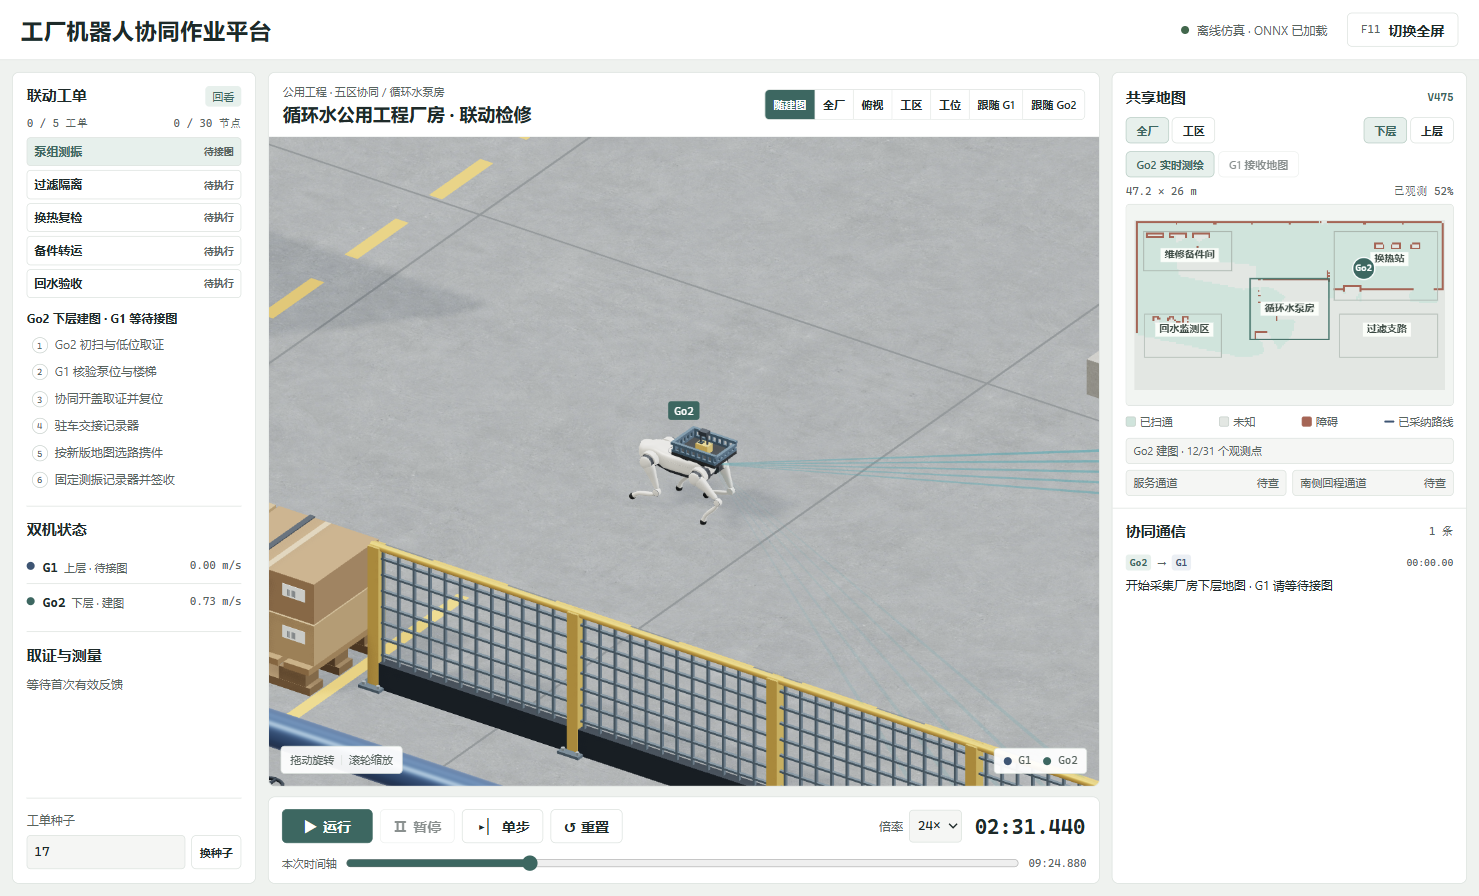
\includegraphics[width=\linewidth,height=0.22\textheight,keepaspectratio]{../assets/factory-map-follow-go2.png}
  {\footnotesize\captionof{figure}{建图时镜头跟随 Go2，右侧更新下层地图。G1 接图后，镜头跟随最近发出消息的机器人。}\label{fig:follow-go2}}
\end{minipage}

\clearpage

\section{设计图与场景建模}

项目前期调用 ImageGen 技能生成了五工区全厂与双层泵房的多视角设计参考图（分别见图~\ref{fig:factory-design} 和图~\ref{fig:pump-design}），以及操作台设计稿与混凝土地面纹理。全厂参考图用来核对设备分区布局与地面安全黄线，泵房参考图则确定了平台格栅、低位管架与检修工装的细部结构。

三维建模阶段对照这些设计图，在场景中补全了夹层与楼梯踏步的格栅纹理、移动检修车的抽屉与脚轮、开放式备件货架，以及过滤、换热与回水设备的管接头和支座。软件把视觉渲染与物理计算分给两个模块承担，Three.js 依据统一的厂房坐标系绘制标线与设备外观细节，MuJoCo 则依据同套坐标下的简化几何体完成碰撞检测与激光测距。

\begin{figure}[!ht]
  \centering
  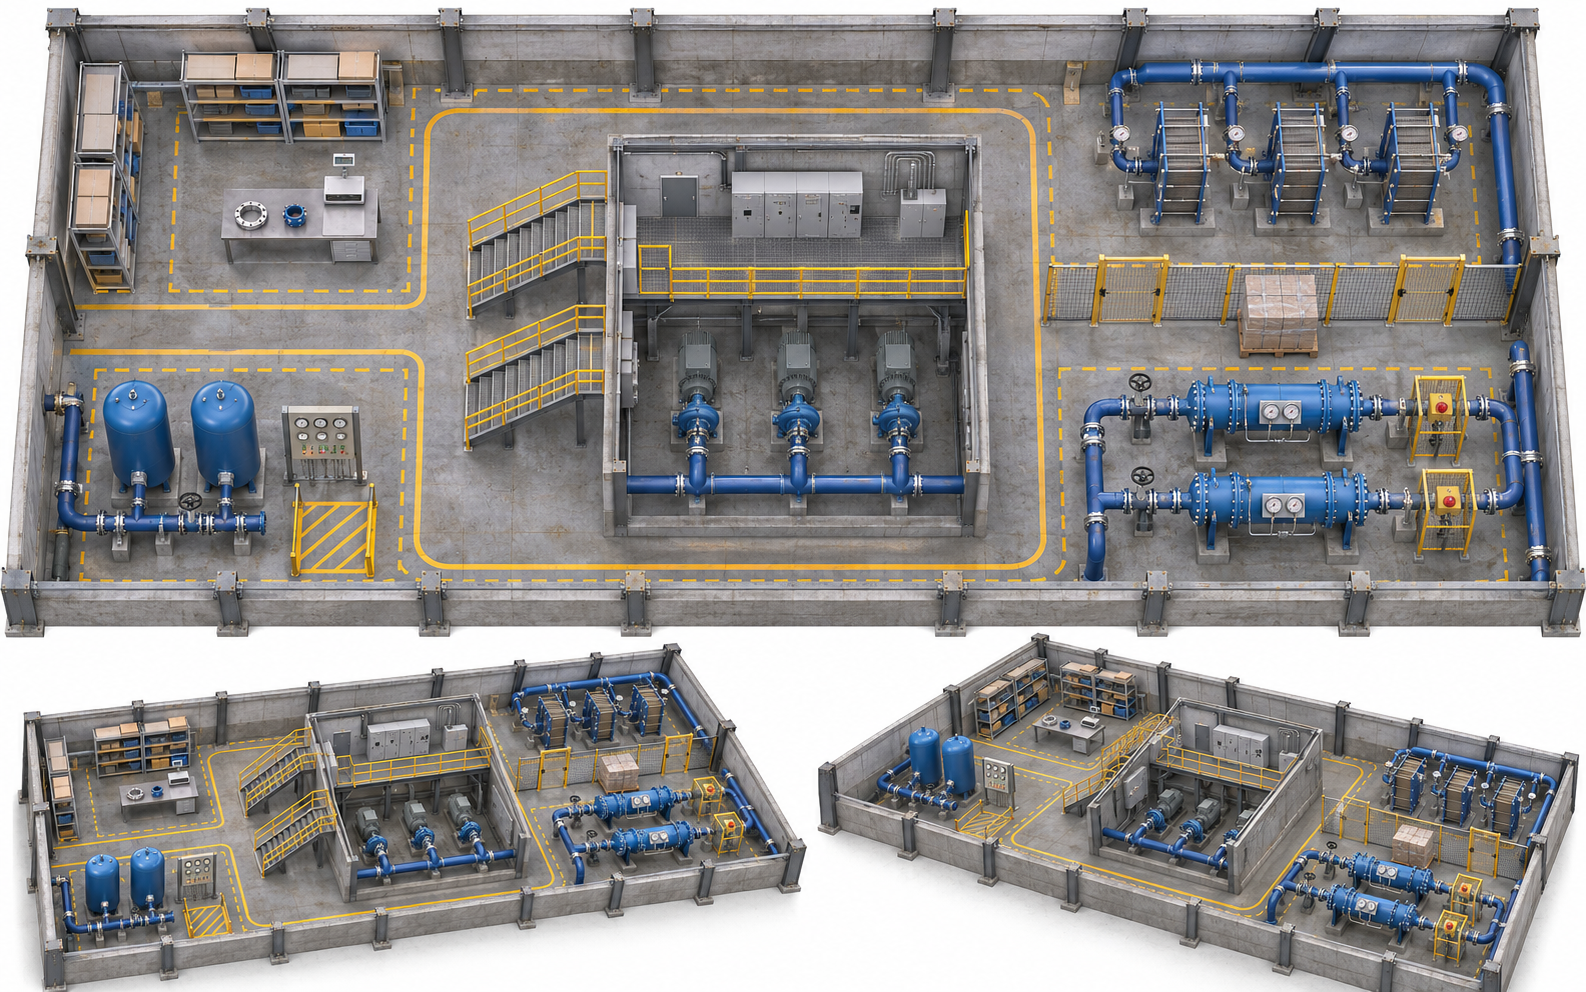
\includegraphics[width=0.98\linewidth,height=0.33\textheight,keepaspectratio]{../assets/imagegen/maps/factory-utility-hall.png}
  \caption{五工区厂房设计参考图。上部是全厂平面，下部是两个斜向剖视。}
  \label{fig:factory-design}
  \par\vspace{6pt}
  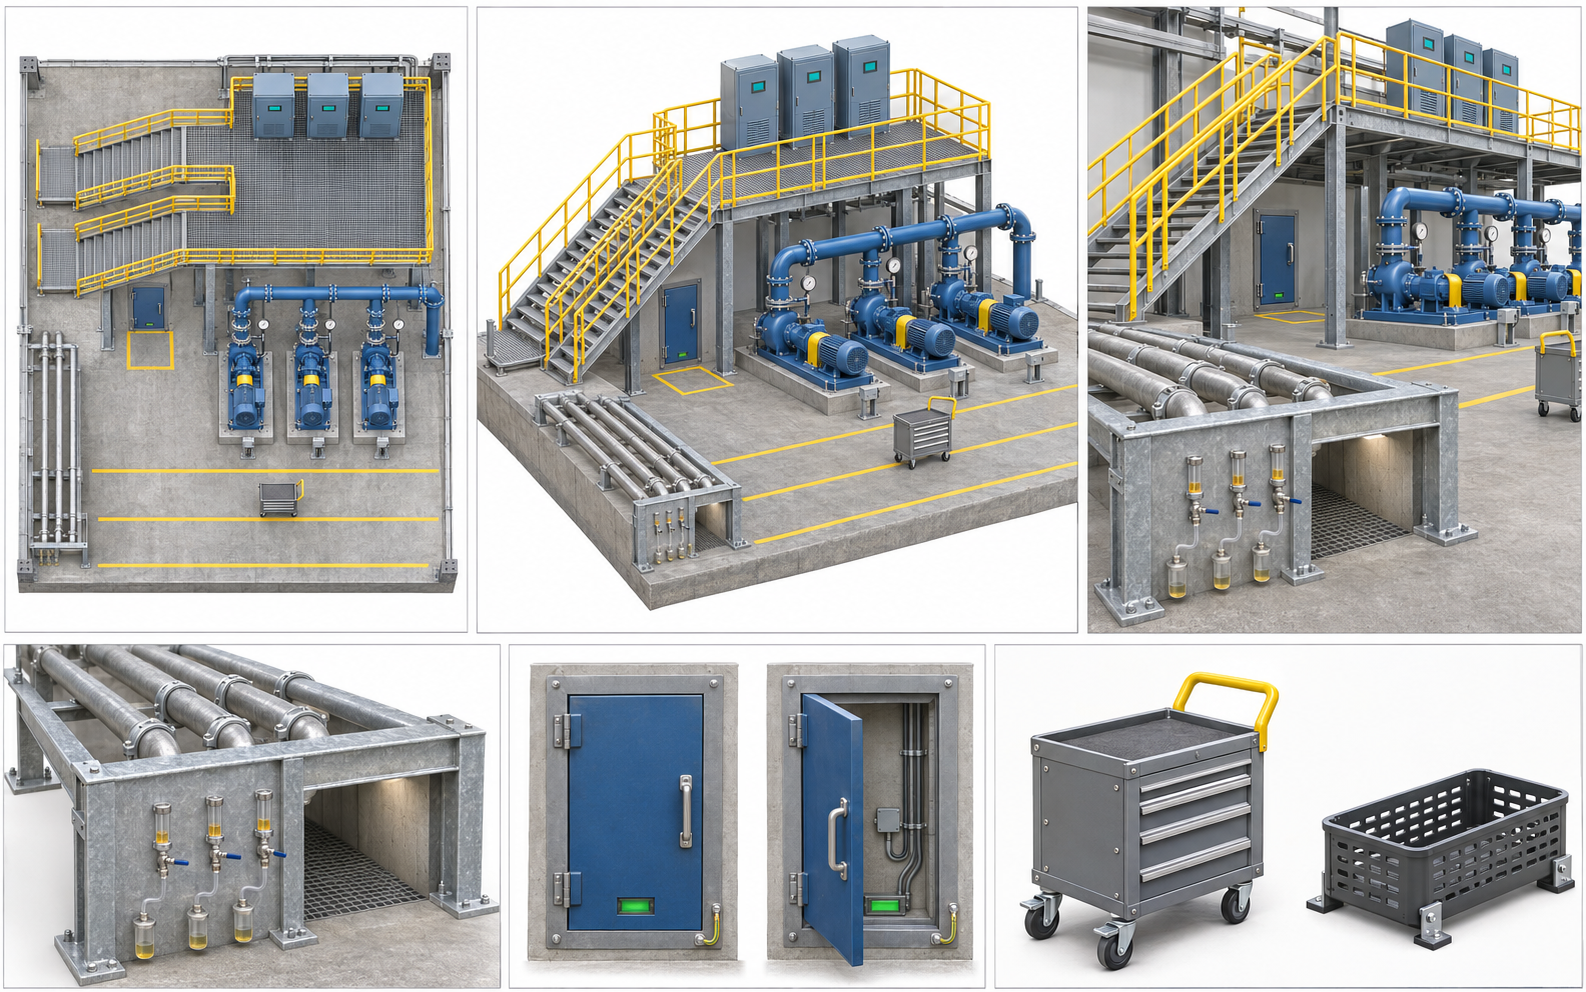
\includegraphics[width=0.98\linewidth,height=0.33\textheight,keepaspectratio]{../assets/imagegen/maps/pump-cooperation-map.png}
  \caption{双层泵房设计参考图。上部呈现泵房上下层空间布局，底部依次放大展示低位管架、检修观察盖、移动检修车与背负式箩筐。}
  \label{fig:pump-design}
\end{figure}

\clearpage

\section{泵房开盖与过滤转场}

默认工单种子为 \texttt{17}。泵组测振工单识别到的异常泵位是 P2。Go2 从低处检查时发现指示片被检修盖挡住，便发消息请 G1 开盖。G1 打开并扶住盖子，Go2 看清绿色指示片后退出观察位（图~\ref{fig:cover}）。

测振签收后，G1 用 Go2 交付的下层地图 \MapVersion{} 规划路线，前往过滤支路（图~\ref{fig:filter-route}）。沿时间轴回看时，机器人姿态、测量读数和消息都对应所选时刻。

\begin{figure}[!ht]
  \centering
  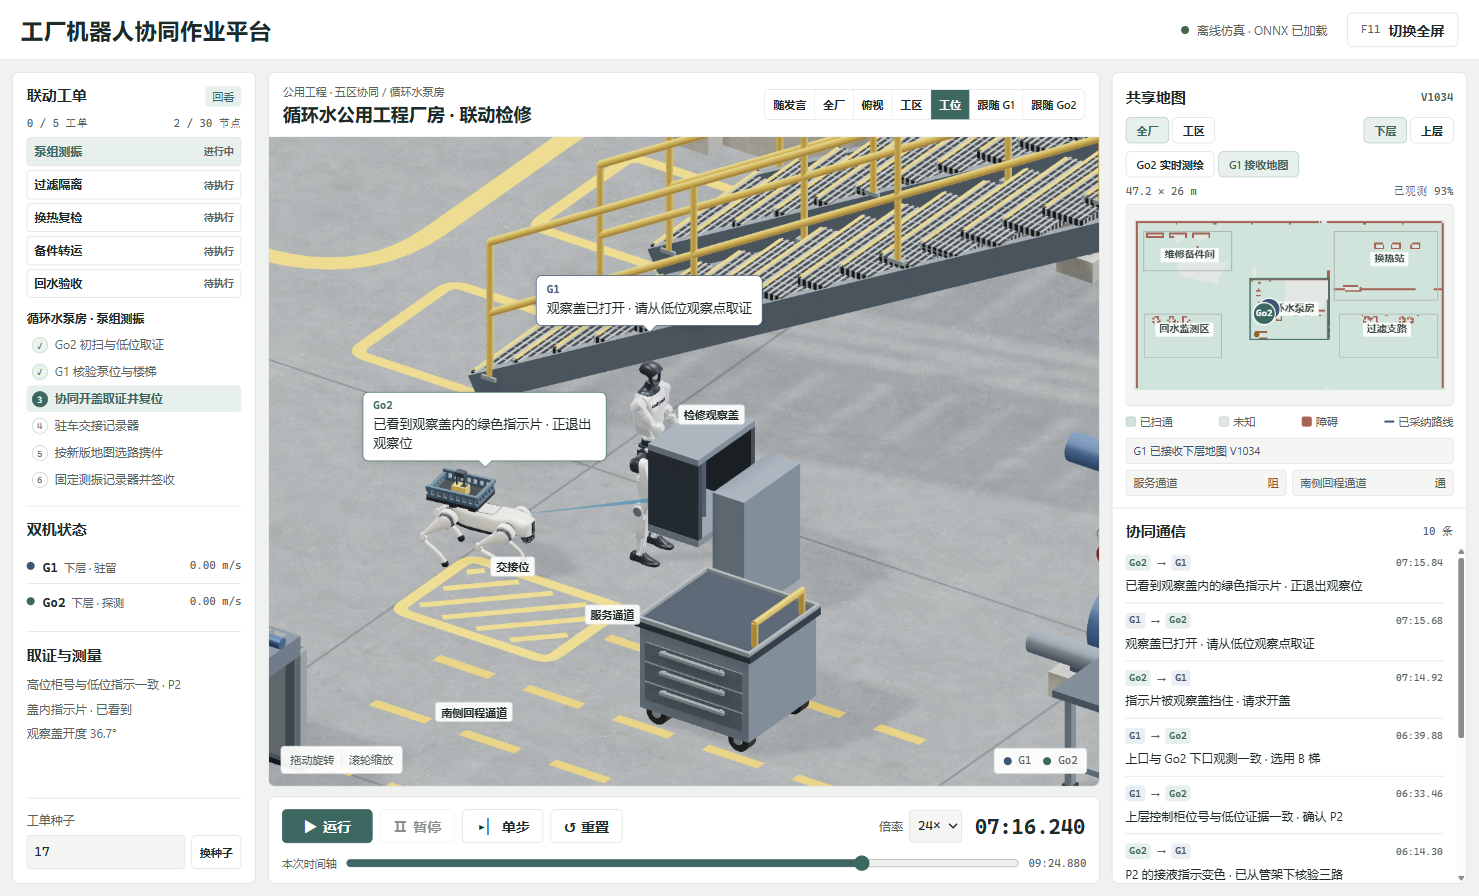
\includegraphics[width=0.97\linewidth,height=0.33\textheight,keepaspectratio]{../assets/factory-pump-cooperation.png}
  \caption{泵组测振。左侧读数显示此时观察盖开度为 $36.7^\circ$。}
  \label{fig:cover}
  \par\vspace{8pt}
  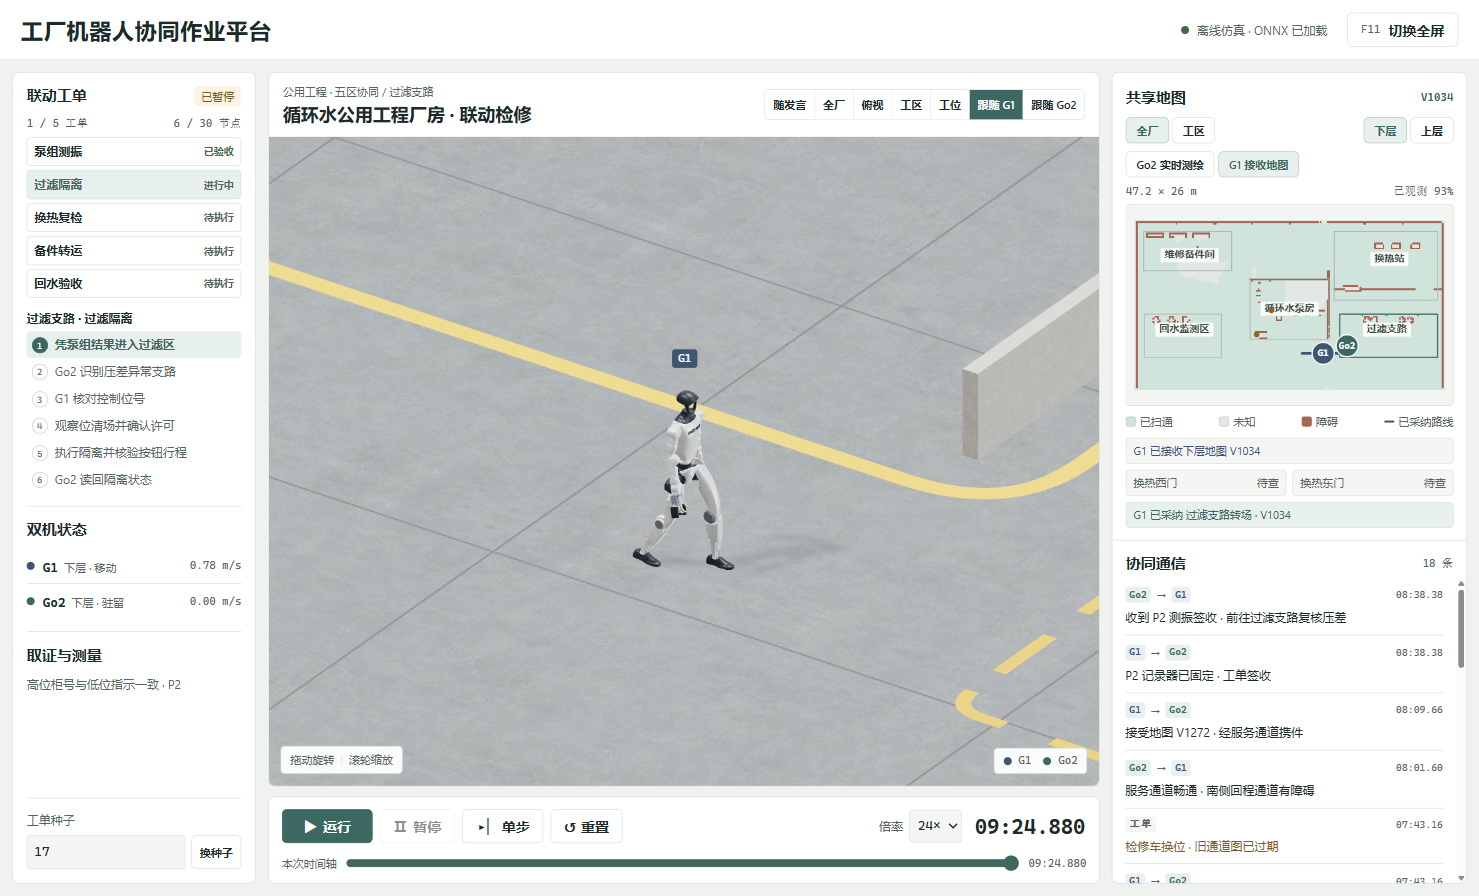
\includegraphics[width=0.97\linewidth,height=0.33\textheight,keepaspectratio]{../assets/factory-g1-map-route.png}
  \caption{过滤转场。蓝线标出 G1 的路线，左侧显示此刻速度为 0.78\,m/s。}
  \label{fig:filter-route}
\end{figure}

\clearpage

\section{开发记录与仿真验证}

\subsection{主要改动}

从早期单泵房原型演进至五工区完整厂房场景的阶段性改动汇总见表~\ref{tab:milestones}。

\begin{table}[htbp]
  \centering
  \small
  \caption{从泵房原型到完整厂房场景的迭代记录}
  \label{tab:milestones}
  \begin{tabularx}{\textwidth}{@{}>{\bfseries\color{DeepTeal}}l X@{}}
    \toprule
    开发阶段 & 主要改动 \\
    \midrule
    泵房原型 & 加入 G1 下楼动作、Go2 低位通行及双机避碰逻辑 \\
    厂房扩建 & 以原泵房为中心扩展至 5 个工区，打通区间连接通道 \\
    设备与标线 & 统一全厂坐标系，校准过滤支路与回水监测区的设备位置、地面黄线与作业点 \\
    工序交接 & 接入协同消息回执机制、三维消息气泡与随发言自动切换的镜头控制 \\
    激光探测 & 实现探测射线可视化，并过滤被 Go2 机身、腿部及箩筐遮挡的无效测量 \\
    地图交付 & 新增下层建图覆盖率校验，支持 G1 依据所接收栅格版本自主规划路线 \\
    \bottomrule
  \end{tabularx}
\end{table}

\subsection{测试结果}

在默认种子 \texttt{17} 的仿真中，Go2 第 \MapTime{} 发出下层地图 \MapVersion{}，当时覆盖率为 \MapCoverage{}。G1 第 345 秒确认收图，随后用此图去过滤支路。经换热东门时，G1 用的是 Go2 复查后发来的 V1481。

\begin{itemize}
  \item \textbf{完整工单}\quad 用 \texttt{0}、\texttt{11}、\texttt{14} 和 \texttt{17} 四个种子各运行一次。每次均完成 5 张工单、30 个节点，G1 两段路线使用各自收到的地图版本。接触监测未记录异常接触。
  \item \textbf{缺项测试}\quad 分别模拟未收到首次下层地图、换热入口新图和回水验收许可。仿真在需要该项数据或许可的工序停下。
  \item \textbf{桌面交互}\quad 在 Windows 发行版上检查了双击启动、默认全屏、\texttt{F11} 切换窗口、建图镜头跟随及时间轴回看。
\end{itemize}

\begin{thebibliography}{9}
  \small
  \bibitem{todorov2012mujoco}
  Emanuel Todorov, Tom Erez, Yuval Tassa.
  MuJoCo: A Physics Engine for Model-Based Control.
  IEEE/RSJ International Conference on Intelligent Robots and Systems (IROS), 2012, DOI 10.1109/IROS.2012.6386109, \url{https://www.roboti.us/lab/papers/TodorovIROS12.pdf}.

  \bibitem{liao2026supermimic}
  Qiayuan Liao, Yiyang Shao, Junfeng Long, Kevin Zakka, Roberto Horowitz, Pieter Abbeel, Koushil Sreenath.
  SuperMimic: Scaling Humanoid Whole-Body Control with One Differentiable World Model.
  Conference on Robot Learning (CoRL), 2026 / arXiv:2610.28480, \url{https://arxiv.org/abs/2610.28480}.

  \bibitem{unitreeGo2}
  Unitree Robotics.
  Go2 官方规格（L2）, \url{https://www.unitree.com/go2/}（访问 2026-11-25）.

  \bibitem{elfes1989occupancy}
  Alberto Elfes.
  Using Occupancy Grids for Mobile Robot Perception and Navigation.
  IEEE Computer, 22(6), 1989, 46--57, DOI 10.1109/2.30720, \url{https://doi.org/10.1109/2.30720}.

  \bibitem{hart1968astar}
  Peter E. Hart, Nils J. Nilsson, Bertram Raphael.
  A Formal Basis for the Heuristic Determination of Minimum Cost Paths.
  IEEE Transactions on Systems Science and Cybernetics (TSSC), 4(2), 1968, 100--107, DOI 10.1109/TSSC.1968.300136, \url{https://doi.org/10.1109/TSSC.1968.300136}.
\end{thebibliography}

\end{document}
